\newpage
\section{Discussion} \label{sec:discussion}

\subsection{Escaping and sparse reward}

Recall that the reward function are defined as:
\begin{equation*}
    \mathcal{r}(s_t, a_t) = \begin{cases}
    \mathcal{r}_\text{goal}, &\text{if $d_t < d_\text{th}$}\\
    \mathcal{r}_\text{obstacle}, &\text{if $x_t < x_\text{th}$}\\
    c (d_t - d_{t-1}), &\text{otherwise.}
    \end{cases}
\end{equation*}
The last case encourages the agent to approach the goal. However, it assumes that there is no long barrier between the agent and the goal. A long obstacle would mean that the agent has to move a distance away from the goal in order to escape it before having a chance to approach the goal. Using this reward function does not give the policy the ability to escape, but it is very difficult to define a reward that can encourage escaping.

On the other hand, the last case can be interpreted as a vague expectation of the terrain on which the agent will be trained, which is a prior knowledge. Essentially, this is no different from the map-based method of building a map before navigation.

Removing the last case results in a reward function that can generate a more ideal reward signal. However, the reward generated by this type of reward function belongs to sparse reward.
\begin{equation*}
    \mathcal{r}(s_t, a_t) = \begin{cases}
    \mathcal{r}_\text{goal}, &\text{if $d_t < d_\text{th}$}\\
    \mathcal{r}_\text{obstacle}, &\text{if $x_t < x_\text{th}$}
    \end{cases}
\end{equation*}
Sparse reward means the agent may only receive positive feedback after completing a long sequence of actions. This can slow down the learning process, as the agent has to explore a large space of possible actions before finding a rewarding state. When using algorithms with poor exploration capability, such as TD3, the agent often learns to stay still after training for a period of time. This is because in the initial stage, it did not explore that reaching the goal would receive a big positive feedback, while moving around aimlessly would receive small negative feedback. Therefore, for the agent, staying still is the way to obtain the highest reward.

Even if the last case is not removed, the reward curve is still difficult to converge and stabilise at the highest point, as shown in Figure \ref{fig:fluctuated}. Although the frequency of reaching the high point increases with the number of training iterations, the episodic return curve brought by a well-defined reward function should typically slowly converge to the highest point and hold steady, rather than fluctuating frequently.
\begin{figure}[htbp]
   \centering
   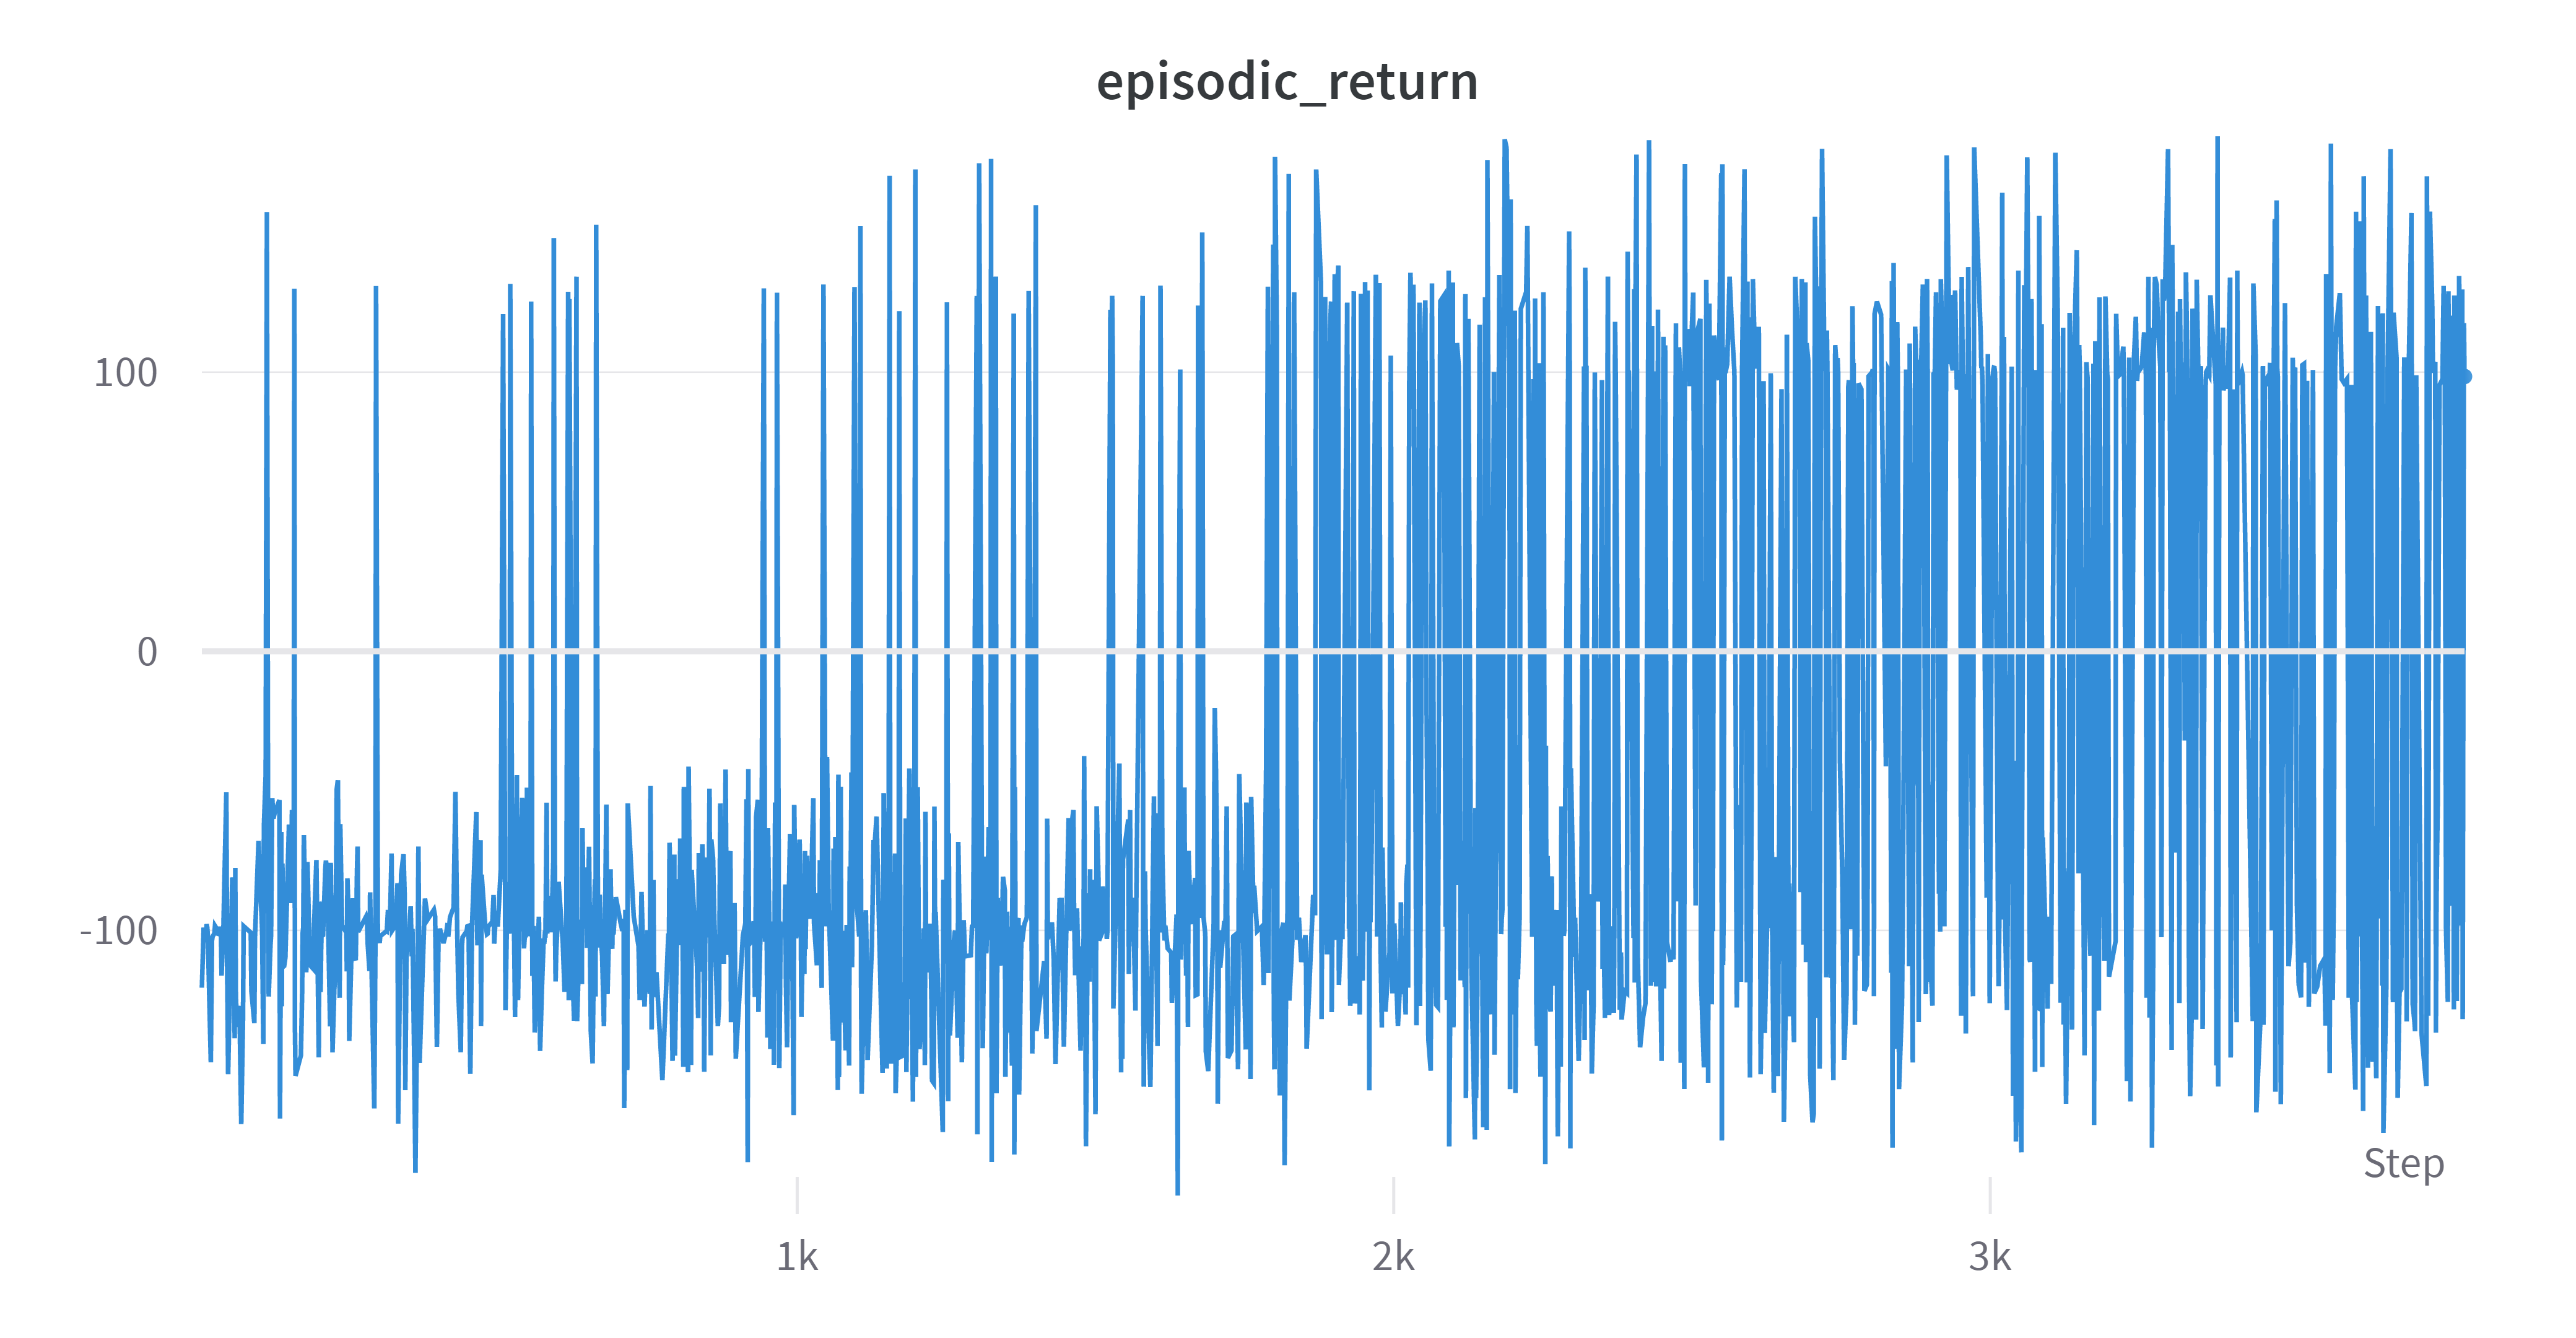
\includegraphics[width=\textwidth]{fluctuated.png}
   \caption{Episodic return curve is fluctuated between the highest and lowest return.}
   \label{fig:fluctuated}
\end{figure}

The ideal DRL algorithm should not heavily rely on a well-defined reward function to learn expected behaviours. We have the above discussion is because the current DRL algorithms are far from idealism and are often depend heavily on reward shaping.

The ideal DRL algorithm should be able to learn expected behaviours effectively without an over-reliance on a well-defined reward function \cite{ref:drl-that-matters}. This is a crucial aspect to consider, as it allows the algorithm to be more adaptable and robust in real-world situations where the environment and desired outcomes are not always clearly defined. The reason of emphasising the importance of moving towards such an ideal algorithm is that, as it was discussed above, current DRL algorithms often relying heavily on reward shaping to guide their learning process.

\subsection{Partial observability}

Normally, in robotic tasks, the agent does not have complete access to the underlying state of the environment. In the case of this project, the agent was only aware of the relative position of the goal, the depth data of it surrounding from LiDAR, and the IMU data. This partial observability can make it difficult for DRL algorithms to learn optimal policies since the agent is not fully aware of its surroundings. From the experimental results, it can be observed that the agent often moves forward and backward multiple times without generate any meaningful movement that helps to achieve the goal. One possible explanation could be that the agent is unaware of its current motion state because the information about the velocity command executed in the previous state is not included in its state space. As the agent does not know whether it was moving forward or backward or turning in the previous state, it can only assess the current situation and generate a new velocity command that is independent of the previous motion state.

\subsection{Transfer learning}

Transfer learning is the ability to leverage knowledge acquired in one task or domain to improve performance in another related task or domain. Currently, DRL algorithms struggle to transfer knowledge across tasks or even across different instances of the same task, requiring extensive retraining. Due to this limitation, in this project, the policy is trained from scratch for every experiment, which wastes a great amount of time.

\subsection{Catastrophic forgetting}

Catastrophic forgetting describes the phenomenon where an artificial neural network optimised by backpropagation has a tendency to suddenly and severely lose memory of previously acquired knowledge when it learns new information. Figure \ref{fig:catastrophic-forgetting} shows a typical example. At the beginning of the training, the TD3 agent mastered the control of the double inverted pendulum within 1k episodes. However, after continued training, at around 5k episodes, the episodic return curve suddenly dropped to nearly zero, indicating that the previously learned knowledge was completely forgotten. After this phenomenon occurred, it took the agent nearly 10k episodes to re-learn how to control the pendulum, and the control policy re-learned was worse than the one learned the first time, as can be seen from the frequency of the curve fluctuations.

\begin{figure}[htbp]
   \centering
   \includesvg[width=\textwidth,pretex=\footnotesize]{InvertedDoublePendulum_episodic_return}
   \caption{Catastrophic forgetting of a TD3 agent trained on the MuJoCo InvertedDoublePendulum environment.}
   \label{fig:catastrophic-forgetting}
\end{figure}
